\documentclass[12pt]{article}

\usepackage{amsmath}
\usepackage{amssymb}
\usepackage{amsthm}
\usepackage{graphicx}
\usepackage{float}

\title{A Model For Quadric Surfaces\\Using\\Geometric Algebra}
\author{Spencer T. Parkin}

\newcommand{\G}{\mathbb{G}}
\newcommand{\V}{\mathbb{V}}
\newcommand{\Vb}{\mathbb{\overline{V}}}
\newcommand{\W}{\mathbb{W}}
\newcommand{\R}{\mathbb{R}}

\newtheorem{theorem}{Theorem}[section]
\newtheorem{definition}{Definition}[section]
\newtheorem{corollary}{Corollary}[section]
\newtheorem{identity}{Identity}[section]
\newtheorem{lemma}{Lemma}[section]
\newtheorem{result}{Result}[section]

\numberwithin{equation}{section}

\author{Spencer T. Parkin}

\begin{document}
\maketitle

\begin{abstract}
Inspired by the conformal model of geometric algebra,
a similar model of geometry is developed for the set
of all quadric surfaces in $n$-dimensional space.  Bivectors of the geometric algebra
are found to be representative of quadric surfaces.  Coordinate free canonical forms
of such bivectors are found for common quadric surfaces.  The model is investigated
for usefulness and compared to the conformal model.
\end{abstract}

\section{The Construction Of The Model}

The stage for this model of $n$-dimensional quadric surfaces is set in the geometric
algebra we'll denote by $\G$ that is generated by a vector space $\W$ of dimension
$2(n+1)$.  Letting $\{e_i\}_{i=0}^{2n+1}$ be an orthonormal set of basis vectors
generating $\W$, we let $\{e_i\}_{i=0}^n$ be such a set of vectors generating
the $(n+1)$-dimensional vector sub-space $\V$ of $\W$ upon which we'll impose the
usual interpretation of $(n+1)$-dimensional homogeneous space.  Specifically,
a vector $v\in\V$ with $v\cdot e_0\neq 0$ represents the point given by\footnote{Throughout this
paper we let the outer product take precedence over the inner product, and the geometric product
take precedence over both the inner and outer products.}
\begin{equation}
e_0\cdot\frac{e_0\wedge v}{e_0\cdot v}
\end{equation}
in $n$-dimensional Euclidean space, imposing the usual correlation between $n$-dimensional
vectors and $n$-dimensional points\footnote{The correlation between
vectors and points spoken of here is that of having a vector represent the point
at its tip when its tail is placed at the origin.}.  We will take the liberty of letting vectors $v\in\V$ with $v\cdot e_0=0$
represent points under the same interpretation of which has just been spoken, as
well as pure directions with magnitude.  The intended interpretation will be made clear
in the context of our usage.  We will refer to all vectors $v\in\V$ with $v\cdot e_0\neq 0$
as projective points, and such vectors with $v\cdot e_0=0$ as non-projective points
or sometimes directions.

We now introduce a function defined on $\G$ having the outermorphic property.
This means that it is a linear function and that it preserves the outer product.  We will
use over-bar notation to denote the use of this function.  Doing so, for any
element $E\in\G$, we define $\overline{E}$ as
\begin{equation}
\overline{E} = SE\tilde{S},
\end{equation}
where the rotor $S$ is given by
\begin{equation}
S = 2^{-(n+1)/2}\prod_{i=0}^n\left(1-e_ie_{i+n+1}\right).
\end{equation}
As the reader can check, for any integer $i\in[0,n]$, we have $\overline{e_i}=e_{i+n+1}$.
The rotor $S$ simply takes any $k$-vector from the geometric algebra generated
by $\V$ and rotates it into the identical geometric algebra generated by the vector
space complement to $\V$ with respect to $\W$, which we'll denote by $\overline{\V}$, thereby creating an isomorphism
between the two geometric algebras.  This idea can be found in \cite{DoranHestenes93}.
We will find the over-bar notation convenient when perform algebraic manipulations in our model.

We are now ready to give the definition by which we will interpret bivectors in $\G$
as $n$-dimensional quadric surfaces.
\begin{definition}\label{def_quadric}
For any element $E\in\G$, we say that $E$ is representative of the $n$-dimensional
quadric surface generated by the set of all projective points $p\in\V$ such that
\begin{equation}\label{equ_quadric_condition}
0 = p\wedge\overline{p}\cdot E.
\end{equation}
\end{definition}
Notice that when $\mbox{grade}(E)>1$, there is no ambiguity, despite the non-associativity
of the inner product, in rewriting equation
\eqref{equ_quadric_condition} as
\begin{equation}
0 = p\cdot E\cdot\overline{p},
\end{equation}
which resembles a sort of conjugation of $E$ by $p$.  This may perhaps be a more
familiar form for readers familiar with the study of quadric surfaces in projective geometry.
Also notice that we have not required that $E$ be a bivector in Definition~\ref{def_quadric},
because we may find this condition useful and meaningful for any element of $\G$.  For now,
however, we will restrict our attention to the case when $E$ is a bivector.

To see why Definition~\ref{def_quadric} works, simply notice that when $E$ is a bivector, we have
\begin{equation}\label{equ_homogeneous_polynomial}
p\wedge\overline{p}\cdot E=-\sum_{i=0}^n\sum_{j=i}^n \lambda_{ij}(p\cdot e_i)(p\cdot e_j),
\end{equation}
which we can recognize as a homogeneous polynomial of degree 2 in the vector components of $p$.
The scalars $\lambda_{ij}$, with $0\leq i\leq j\leq n$, may be formulated in terms of $E$ by
\begin{equation}\label{equ_quadric_components}
-\lambda_{ij} = \left\{\begin{array}{ll}
e_i\overline{e_j}\cdot E & \mbox{if $i=j$,} \\
\left(e_i\overline{e_j}-\overline{e_i}e_j\right)\cdot E & \mbox{if $i\neq j$.}
\end{array}\right.
\end{equation}
It should be noted that bivectors do not uniquely represent quadric surfaces, not even up to scale.
This is apparent from equation \eqref{equ_quadric_components} when we see that for $i\neq j$,
we can freely choose certain components of the bivector without changing the represented
quadric so long as that their sum is still $-\lambda_{ij}$.  The problem this may pose in our model
comes from a very important result in the conformal model.  In the conformal model, if
two blades are known to represent the same non-trivial geometry in the same way, then it can be shown that the
two blades are equal, up to scale.  In our present model, it may take more than just
homogenization to get a bivector known to represent a certain geometry in a
known canonical form.  To account for this during the performance of algebraic manipulations,
we will introduce the following notation.  We will say that quadrics $E_a$ and $E_b$ are
equivalent, writing $E_a\equiv E_b$, whenever $E_a$ and $E_b$ represent the same quadric
under Definition~\ref{def_quadric}.  For example, for any two vectors $u,v\in\V$, we have
\begin{equation}
u\wedge\overline{v}\equiv -2u\wedge\overline{v}\equiv u\wedge\overline{v}+v\wedge\overline{u}
\equiv(u+\overline{v})\wedge(u-\overline{v}).
\end{equation}

Another important difference to point out here between our present model and the conformal model is that,
unlike what we can analogously expect from the point-definition of the conformal model,
here the 2-blade form $a\wedge\overline{a}$ found in Definition~\ref{def_quadric}, for
any projective point $a\in\V$ not at origin, does not represent the projective point $a$ under Definition~\ref{def_quadric}.
In homogenized form, the projective point represented by $a\wedge\overline{a}$ is given by
\begin{equation}
e_0 - \left(e_0\cdot\frac{e_0\wedge a}{e_0\cdot a}\right)^{-1},
\end{equation}
which is the reflection about the origin of the spherical reflection of the projective point $a$
about the unit-sphere centered at the origin.  The projective point $e_0$ at the origin
simply represents the empty point-set geometry, or the geometry of nothing.  It is also
easy to see that $a\wedge\overline{a}$ cannot represent itself, because there are no
null blades in our purely Euclidean geometric algebra $\G$.

\section{The Construction Of Quadric Surfaces In The Model}

Having constructed our model, we are now ready to find canonical forms of bivectors
representing a variety of well-known quadric surfaces.  Our approach here will be
similar to that taken in Section 3 of \cite{Miller87}.

Let us begin with the
spheroid, (a special case of ellipsoid), the circular cylinder, and the circular hyperboloid
of one sheet.  We will find that all of these surfaces share the same canonical form,
because they may all be characterized as the non-projective point solution set of the equation
\begin{equation}\label{equ_spheroid}
0 = -r^2 + (x-c)^2 + \lambda((x-c)\cdot v)^2
\end{equation}
in the non-projective point $x\in\V$, where $c\in\V$ is a non-projective
point denoting the center of the surface, $v\in\V$ is a unit-length direction
vector, $r\in\R$ is the radius of the geometry about the axis $v$ at $c$, and
$\lambda\in\R$ is a scalar indicating the type and extremity of the surface.
Specifically, if $\lambda<-1$, we get a circular hyperboloid of one sheet,
if $\lambda=-1$, we get a circular cylinder, if $-1<\lambda<0$, we get a stretched
sphere, if $\lambda=0$, a sphere, and if $\lambda>0$, a squished sphere.  Interestingly,
when $r=0$ and $\lambda<-1$, we get circular conical surfaces; a right-circular conical
surface if $\lambda=-2$.

Expanding equation \eqref{equ_spheroid}, we get
\begin{equation}
0 = x^2 + \lambda(x\cdot v)^2 - 2x\cdot (c+\lambda(c\cdot v)v) + c^2 + \lambda(c\cdot v)^2 - r^2,
\end{equation}
from which it is possible to factor out $-p\wedge\overline{p}$
in terms of the inner product, where $p=e_0+x$
is a homogenized projective point.  Doing so, we see that the bivector
$E$ given by
\begin{equation}\label{equ_spheroid_bivector}
E = \Omega + \lambda v\wedge\overline{v} - 2(c+\lambda(c\cdot v)v)\wedge\overline{e_0} + (c^2+\lambda(c\cdot v)^2-r^2)A,
\end{equation}
is representative of the three surface types by Definition~\ref{def_quadric}, where the constant
$\Omega$ is defined as
\begin{equation}
\Omega=\sum_{i=1}^n e_i\overline{e_i},
\end{equation}
and $A$ is the constant defined as $A=e_0\overline{e_0}$.  We will find each of these useful as
frequently recurring constants in our calculations.

Such forms as that in equation \eqref{equ_spheroid_bivector} are useful, not only
for composition, but especially decomposition in the cases
where we have formulated what may, for example, be a spheroid by some means
other than composition.
This gives the model power as an analytical tool.  If we can solve a problem whose solution
is a bivector known to represent a spheroid, then we can use this canonical form to answer
questions about that spheroid.  Where is its center?  What is its axis?  What is its radius
about that axis?  As is often the case in mathematics, however, decomposition is
harder than composition.  A general sequence of decomposition steps for the
form \eqref{equ_spheroid_bivector} is not obvious, if it exists, but we will
proceed now to give such a sequence for the case when $E$ is known
to be a cylinder.  That is, when $\lambda=-1$.

The first thing to notice is that the canonical form $E$ in equation \eqref{equ_spheroid_bivector}
is in a homogenized form, because the coeficient of $\Omega$ is 1.  If our given bivector
is not already homogenized, then we'll want to divide it through by $-\Omega\cdot E/n$.

We then notice that for $1\leq i<j\leq n$, we have the system of equations
\begin{equation}
(v\cdot e_i)(v\cdot e_j) = -e_i\overline{e_j}\cdot E,
\end{equation}
from which we can deduce the magnitudes of the components of $v$ and the
direction of $v$, up to sign.  For example, if $(v\cdot e_i)(v\cdot e_j)>0$,
then $\mbox{sign}(v\cdot e_i)=\mbox{sign}(v\cdot e_j)$, and so on.
It is also helpful to notice that for all $i=j$, we have
\begin{equation}
(v\cdot e_i)^2 = -1 - e_i\overline{e_j}\cdot E.
\end{equation}
It is unfortunate that we had to refer to a basis to obtain $v$; nevertheless,
it is done.  The rest of the decomposition will proceed with greater satisfaction.

There is no way to recover $c$ for cylinders, which is quite obvious.
The choice for the point $c$, the center of the cylinder, may be arbitrarily
chosen as any point along its spine.  This information is lost in composition,
so we may therefore arbitrarily choose
\begin{equation}
c=-A\cdot(E\wedge e_0)/2
\end{equation}
as the cylinder's center, which, incidentally, will also be the point on the spine of
the cylinder closest to the origin.

Lastly, we may find the radius of the cylinder from the simple equation
\begin{equation}
r^2 = c^2 + A\cdot E.
\end{equation}

A generalization of equation \eqref{equ_spheroid} should be mentioned
before moving on.  It is given by
\begin{equation}
0 = -r^2 + (x-c)^2 + \sum_{i=1}^k \lambda_i((x-c)\cdot v_i)^2,
\end{equation}
which would probably give us the general set of ellipsoids, provided
the set of $k$ direction vectors in $\{v_i\}_{i=1}^k$ are
linearly independent.

The following table summarizes a few additional canonical forms.
\begin{equation}\label{equ_canonical_forms_table}
\begin{array}{|l|l|}
\hline
\mbox{Geometry} & \mbox{Canonical/Homogenized Form} \\
\hline
\mbox{Plane} & v\wedge\overline{e_0} - (c\cdot v)A,\;|v|=1 \\
\hline
\mbox{Sphere} & \Omega - 2c\wedge\overline{e_0} + (c^2-r^2)A \\
\hline
\mbox{Point} & \Omega - 2c\wedge\overline{e_0} + c^2A \\
\hline
\mbox{Line} & \Omega - v\wedge\overline{v} - 2u\wedge\overline{e_0} + u^2A,\;u=c-(c\cdot v)v \\
\hline
\mbox{Cylinder} & \Omega - v\wedge\overline{v} - 2u\wedge\overline{e_0} + (u^2-r^2)A,\;u=c-(c\cdot v)v \\
\hline
\mbox{Plane-Pair} & ((c_a\cdot v_a)e_0-v_a)\wedge((c_b\cdot v_b)\overline{e_0}-\overline{v_b}) \\
\hline
\end{array}
\end{equation}
The plain-pair form is discussed below with equation \eqref{equ_double_plane}.  Here,
in table \eqref{equ_canonical_forms_table}, $c_a,c_b\in\V$ are non-projective points
on the two planes, and $v_a,v_b\in\V$ are direction vectors normal to each of the two planes.

\section{Making Use Of The Model}

Admittedly, there is really nothing interesting about this model unless we can
prove that it has some utility.  The conformal model, for example, has at least
two great features.  The first is the utility of the wedge product in generating
intersections between geometries in dual form, or point-fitting between
geometries in direct form.  A good user of the conformal model can even
make use of dual imaginary intersections by reinterpreting them as real geometries
in direct form.  The second great feature of the conformal model is the
surprising fact that all geometries in the conformal model are also, as versors, conformal transformations
with geometric significance relative to the simultaneously represented geometry.
Then, realizing that all conformal geometries, (with the exception of flat points), have
a factorization in direct form as an outer product of points, the outermorphic
property of versor conjugation allows us to predict the action of any versor
transformation on almost any conformal geometry.

These are great features!  But what can the model at present do for us?  Well,
the first observation we must make is that the set of all known quadrics
is represented by the set of all bivectors in $\G$, under-which the inner
and outer products are obviously not closed.  Only addition and subtraction
are closed in this set, and so we're left to wonder what we might be able
to prove about the addition and subtraction of $n$-dimensional quadric surfaces.
Letting $B_a,B_b\in\G$ be bivectors, it is not hard to see that $B_a\pm B_b$, under
Definition~\ref{def_quadric}, must represent at least the intersection, if any,
of the quadric surfaces $B_a$ and $B_b$, but this is not an exact answer to the
question of what surface $B_a\pm B_b$ represents.

Let's try an example.  Suppose $B_a$ and $B_b$ are both homogenized spheres with
a real intersection and having
non-projective centers $c_a,c_b\in\V$, respectively.  Let $r_a,r_b\in\R$
be the respective radii of $B_a$ and $B_b$.  It then follows from
table \eqref{equ_canonical_forms_table} that $B_a-B_b$, in homogenized
form, is given by
\begin{equation}\label{equ_diff_of_spheres}
\frac{v}{|v|}\wedge\overline{e_0}-\left(\frac{v}{|v|}\cdot\frac{c_a+c_b+(r_b^2-r_a^2)v^{-1}}{2}\right)A,
\end{equation}
where $v$ is the vector $c_a-c_b$, which, again by table \eqref{equ_canonical_forms_table},
tells us that this is a plane with normal $v$.  A point on the plane is also apparent from
\eqref{equ_diff_of_spheres}.  Then, knowing that $B_a-B_b$ must contain the intersection of the
two spheres, we can conclude that this point must be in the plane containing the circle that is
the intersection of the two spheres, because $B_a-B_b$ must be the said plane.  Notice
that even if the spheres don't intersect, we still get a meaningful result.  A picture of
$B_a-B_b$ is given in Figure~\ref{fig_diff_of_spheres}.

\begin{figure}
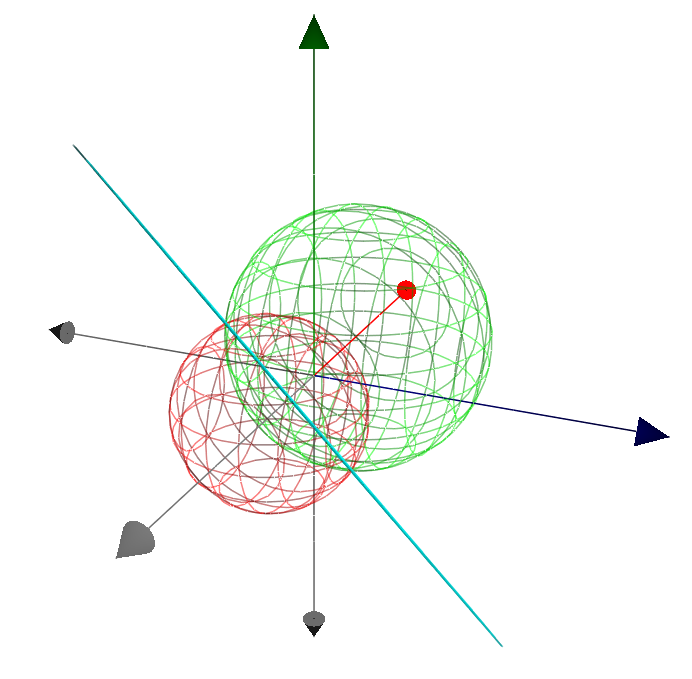
\includegraphics[scale=0.7]{DiffOfSpheres}
\caption{The difference of two spheres gives a plane, shown here on edge.  The spheres were rendered as a number of traces in various parallel planes.}
\label{fig_diff_of_spheres}
\end{figure}

At first sight, the sum of a sphere and a plane may not seem that interesting.
However, the sum of a homogenized sphere and a non-homogenized plane is
interesting, because the result is always a sphere in homogenized form.  The
scalar amount at which the plane is non-homogenized simply indicates half
the length along the normal of the plane that the center of the original sphere
is displaced in the direction of that normal to find a sphere intersecting the
plane in the same circle as that of the original sphere.

Interestingly, the difference of spheres generalizes to the idea of subtracting
spheroids.  A picture of this is given in Figure~\ref{fig_diff_of_spheroids}.
Of course, there is undoubtedly a geometric significance in the difference
between any two homogenized quadric surfaces containing $\Omega$.  It
would be interesting to find out exactly what that is.

\begin{figure}
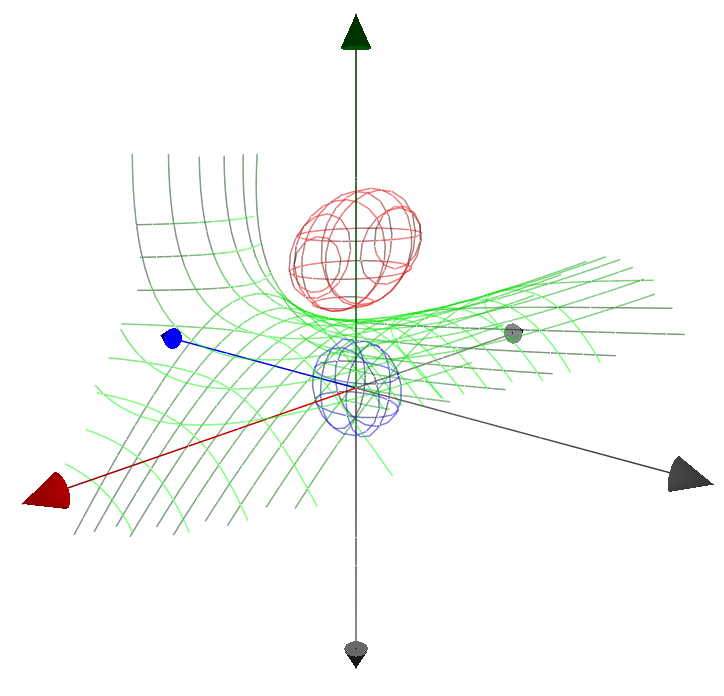
\includegraphics[scale=0.7]{DiffOfSpheroids}
\caption{The difference of two spheroids gives a hyperbolic paraboloid.  Traces in various planes were used to render the surfaces.}
\label{fig_diff_of_spheroids}
\end{figure}

\section{The Consideration Of Trivector Quadrics}

Notice that any trivector $T\in\G$ can be written in the form
\begin{equation}
T = \sum_{i=1}^k v_i\wedge B_i,
\end{equation}
where $\{v_i\}_{i=1}^k\subset\W$ is a set of $k$ vectors and $\{B_i\}_{i=1}^k\subset\G$
is a set of $k$ bivectors.  Applying Definition~\ref{def_quadric}, we get the equation
\begin{equation}\label{equ_trivector_geo}
0 = p\wedge\overline{p}\cdot T =
p\cdot\sum_{i=1}^k(\overline{p}\cdot v_i)B_i -
\overline{p}\cdot\sum_{i=1}^k(p\cdot v_i)B_i +
\sum_{i=1}^k(p\wedge\overline{p}\cdot B_i)v_i.
\end{equation}
Now if $\{v_i\}_{i=1}^k$ was a linearly independent set, and for all projective points $p\in\V$, we have $p\cdot v_i=\overline{p}\cdot v_i=0$
for any integer $i\in[1,k]$, then it is clear
from equation \eqref{equ_trivector_geo} that $T$ represents the intersection of all quadrics in $\{B_i\}_{i=1}^k$.
Unfortunately, it is obviously not possible to satisfy this condition in $\G$ without expanding it.
Doing so, we might introduce two new basis vectors $b_1$ and $b_2$, thereby finding the trivector
$T=b_1\wedge B_1+b_2\wedge B_2$ as representative of the intersection of the quadrics $B_1$ and $B_2$.
This, however, may be undesirable, because $T$ cannot directly characterize the intersection in this form, but
only indirectly as the characterization of the quadrics $B_1$ and $B_2$ taken in the intersection operation.
Such indirect characterizations should not be so easily dismissed, however, because a common theme
in the process of performing geometry in a model based in geometric algebra is the idea of simply transforming
one characterization or interpretation of a given geometry into another.  If we were able to formulate $T$ through some means
other than that of the intersection of $B_1$ and $B_2$, then the original characterization, whatever that may
have been, may be transformed into
this one, thereby providing a new interpretation of the geometry represented by $T$ as the intersection
of the two quadrics $B_1$ and $B_2$.

In any case, we are not going to expand $\G$, because it is already complicated enough as it is, and we
are far from discovering everything possible in the present model imposed upon it.
Let's take a step back for a moment, then, and narrow our scope to that of 3-blades.
Doing so, we see that
what might motivate us to investigate the set of all quadrics that are 2-blades, (or to find
a better model where all quadrics are 2-blades), is the following result.

For any given non-zero 3-blade $T\in\G$, given by $T=a\wedge b\wedge c$, the
geometry represented by this 3-blade under Definition~\ref{def_quadric} is the intersection
of the 3 quadrics $a\wedge b$, $a\wedge c$ and $b\wedge c$.
The proof of this follows directly from the following identity, which the reader can easily verify.
\begin{equation}
p\wedge\overline{p}\cdot a\wedge b\wedge c
 = (p\wedge\overline{p}\cdot a\wedge b)c
 - (p\wedge\overline{p}\cdot a\wedge c)b
 + (p\wedge\overline{p}\cdot b\wedge c)a
\end{equation}
Now realize that since $a\wedge b\wedge c\neq 0$, $\{a,b,c\}$ is a linearly
independent set, and therefore, $0=p\wedge\overline{p}\cdot T$ if and
only if $p$ is on $a\wedge b$, $a\wedge c$ and $b\wedge c$.

This, of course, would generalize to blades of higher grade.  The 3-way intersection
of quadrics was given a great deal of consideration in \cite{ZhiqiangXu05}.
This ability to intersect three quadrics, however, is restrictive in at least
two ways.  First, all three quadrics must be blades.   And secondly, the
three quadrics must pair-wise share a common vector in their respective factorizations.
In any case, the result leads us to a consideration
of quadrics that are 2-blades.  This deserves its own section.

\section{The Consideration Of 2-Blade Quadrics}

Letting $B\in\G$ be a 2-blade of the form
\begin{align}\label{equ_two_blade_quadric}
B &= (a+\overline{b})\wedge(c+\overline{d}) \\
 &= a\wedge c + a\wedge\overline{d} - c\wedge\overline{b} + \overline{b\wedge d} \\
 &\equiv a\wedge\overline{d} - c\wedge\overline{b},
\end{align}
where $a,b,c,d\in\V$, our first observation is that $a\wedge c$ and $\overline{b\wedge d}$ contribute nothing
to the shape of the quadric, because they represent the geometry of all space under
Definition~\ref{def_quadric}, which is easily verified.  What remains is the difference
between two quadrics of the form $u\wedge\overline{v}$, where $u,v\in\V$.  It is
easy to show that a quadric of this form is a double plane.
\begin{equation}\label{equ_double_plane}
0 = p\wedge\overline{p}\cdot u\wedge\overline{v} = -(p\cdot v)(p\cdot u)
\end{equation}
The projective point solution set of equation \eqref{equ_double_plane} is
clearly the union of such a set for the equation $0=p\cdot v$ and $0=p\cdot u$,
both of which are planes.  The plane for $v$ has normal $e_0\cdot e_0\wedge v$,
and the point $e_0-(v\cdot e_0)(e_0\cdot e_0\wedge v)^{-1}$ as the point on the plane closest to the origin.

Returning to \eqref{equ_two_blade_quadric}, it is clear now that $B$ represents
the projective point solution set to the equation
\begin{equation}\label{equ_two_blade_quadric_vector_form}
0 = \left|\begin{array}{cc} p\cdot a & p\cdot b \\ p\cdot c & p\cdot d \end{array}\right|.
\end{equation}
It is not at all immediately obvious as to what type of surface this may be.
What we do know, however, is that it must
contain the intersection, if any, of the two pairs of planes $a\wedge\overline{d}$ and $c\wedge\overline{d}$.
In most cases this is a pair of lines, many instances of which can be seen to fit the surface
given in Figure~\ref{fig_quadric_blade}.

\begin{figure}
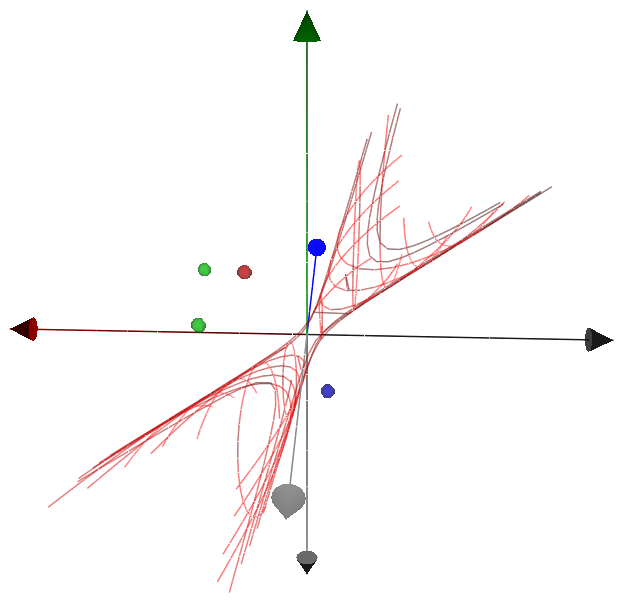
\includegraphics[scale=0.7]{QuadricBlade}
\caption{A quadric formed by four points composing a 2-blade.}
\label{fig_quadric_blade}
\end{figure}

One immediate observation about equation \eqref{equ_two_blade_quadric_vector_form}
is that if all points lie in a plane through the origin, then the equation remains
invariant when $p$ is replaced with $p+v$, where $v\in\V$ is a direction vector
orthogonal to that plane.  This shows that in this case, $B$ must be the
extrusion of a conic section through a dimension parallel to the norm of
the common plane of the four points.  It is not clear whether all conic
sections can be represented this way, though, because certainly not
all quadrics can be represented with a 2-blade.  It may, howerver,
be possible to represent all extruded conic sections with bivectors that are sums
of blades having the property just mentioned.

Lastly, it should be noted that, unlike equation \eqref{equ_double_plane},
equation \eqref{equ_two_blade_quadric_vector_form} is sensative to which
of the four points are homogenized and which are not.  This is something
we would need to carefully consider in any analysis of this equation.

\section{Transformations In The Model}

In this section we finally show that this model has merit with at least one
interesting feature, which is that bivector quadrics can be transformed by
versors in a meaningful way.  Specifically, we can rotate any quadric about
any axis using a carefully formulated rotor.

We begin by observing that for any non-projective point $v\in\V$,
we can easily rotate this point as $Rv\tilde{R}$, where $R$ is
given by
\begin{equation}
R = \cos(\theta/2) - aI\sin(\theta/2),
\end{equation}
where $a\in\V$ is a direction vector, and $I=\prod_{i=1}^n e_i$.  Furthermore,
for any non-projective point $v\in\V$, notice that
\begin{equation}
\overline{v} = R\overline{v}\tilde{R},
\end{equation}
showing that the counter-part $\overline{v}$ of $v$ in $\overline{\V}$ remains invarient
under this rotation.  (The proof of this is similar to the proof we'll give
shortly that $R$ leaves $e_0$ invariant.)  Of course, we can formulate an equivilant of $R$
that will rotate $\overline{v}$, and it is simply $\overline{R}$.  Then, seeing
that $\overline{R}$ leaves $v$ invariant, it follows
that $V=R\overline{R}$ is a rotor that will rotate the 2-blade
$v\wedge\overline{v}$ in the desired way.  Specifically, we have
\begin{equation}
V(v\wedge\overline{v})\tilde{V} = Rv\tilde{R}\wedge\overline{Rv\tilde{R}}.
\end{equation}

Now, for all quadrics
that are sums of blades of the form $a\wedge\overline{b}$, with $a,b\in\V$,
and each of $a$ and $b$ being a non-projective position or direction related to the quadric,
we see that for such quadrics $E\in\G$, the rotation $E'$ of this quadric
about an axis $a\in\V$ by an angle $\theta$, is given by
\begin{equation}
E' = VE\tilde{V}.
\end{equation}
Interestingly, this formula applies to all quadrics, because it can be shown
that $V$ leaves $\Omega$ and $A$ invariant under versor conjugation.
Indeed, a spheroid in the form of equation \eqref{equ_spheroid_bivector}
can be rotated as illustrated in Figure~\ref{fig_rot_spheroid}.
\begin{figure}
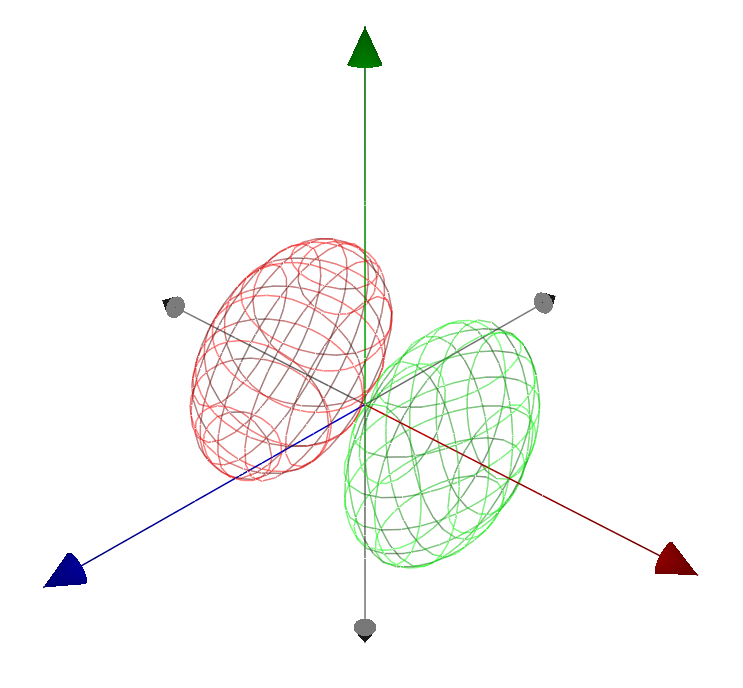
\includegraphics[scale=0.7]{RotatedSpheroid}
\caption{The rotation of a spheroid about the axis $(e_1+e_2+e_3)/\sqrt{3}$ by $\pi$ radians.}
\label{fig_rot_spheroid}
\end{figure}

To see that $V$ leaves $A$ invariant, notice that
\begin{equation}
VA\tilde{V} = Re_0\tilde{R}\wedge\overline{Re_0\tilde{R}}.
\end{equation}
We need only show now that $R$ leaves $e_0$ invariant.  To that end, we see that
\begin{align}
Re_0\tilde{R} &= \cos^2\frac{\theta}{2}e_0 + \cos\frac{\theta}{2}\sin\frac{\theta}{2}(e_0 aI - aIe_0) - \sin^2\frac{\theta}{2}aIe_0aI \\
 &= \cos^2\frac{\theta}{2}e_0 - \sin^2\frac{\theta}{2}(aI)^2 e_0 \\
 &= \left(\cos^2\frac{\theta}{2}+\sin^2\frac{\theta}{2}\right)e_0 = e_0,
\end{align}
since $|a|=1$.  Seeing that $V$ leaves $\Omega$ invariant is a bit trickier.  We first
observe that
\begin{equation}\label{equ_versor_acting_on_omega}
V\Omega\tilde{V} = \sum_{i=1}^n Re_i\tilde{R}\wedge\overline{R e_i\tilde{R}}.
\end{equation}
It is important to realize at this point that for all integers $i\in[1,n]$, that $e_i\neq Re_i\tilde{R}$,
yet $V$ really does leave $\Omega$ invariant.  To see why, we will rewrite $e_i$
in equation \eqref{equ_versor_acting_on_omega} as
\begin{equation}
e_i = \sum_{j=1}^n (e_i\cdot e_j)e_j.
\end{equation}
Now realize that
\begin{equation}
Re_i\tilde{R} = \sum_{j=1}^n (Re_i\tilde{R}\cdot e_j)e_j.
\end{equation}
It then follows that for any integer $i\in[1,n]$, we have
\begin{equation}
-e_i\wedge\overline{e_i}\cdot V\Omega\tilde{V} = \sum_{j=1}^n (Re_i\tilde{R}\cdot e_j)^2 = (Re_i\tilde{R})^2 = 1,
\end{equation}
showing that the coefficient of $e_i\wedge\overline{e_i}$ in $V\Omega\tilde{V}$ is 1.  Realize that
the application of a rotor leaves the magnitude of a vector unchanged.  To finish the proof, we
observe that for all integers $i\neq j$ in $[1,n]$, we have
\begin{equation}
-e_i\wedge e_j\cdot V\Omega\tilde{V} = \sum_{k=1}^n (Re_i\tilde{R}\cdot e_k)(Re_j\tilde{R}\cdot e_k)
= (Re_i\tilde{R})\cdot(Re_j\tilde{R}) = 0,
\end{equation}
showing that the coefficient of $e_i\wedge\overline e_j$ in $V\Omega\tilde{V}$ is 0.  Realize that
the action of a rotor taken with two orthogonal vectors does not change their orthogonal relationship.
It now follows that $V\Omega\tilde{V}=\Omega$.

% Question: What 2-blade form, if any, gives a cylinder?  Clearly it is invariant
% under a rotation about the axis of the cylinder, which means that we can
% show that the 2-blade is invariant under a given rotor, provided that we can
% get the axis of the cylinder to go through the origin.  Interpreting this
% rotation in terms of the sum of the two blades that may form the 2-blade,
% can we show that this is a proof that cylinders are ruled surfaces?
% (Which is a bit dumb, since it's an obvious fact that they are.)
% We might be able to if these two 2-blades are double-planes that
% intersect in real lines.

\section{Concluding Remarks}

While it has been shown that elements of $\G$ do indeed, under a given
definition, represent quadric surfaces, there really is nothing more or less
interesting about adding and subtracting these elements than adding and
subtracting vector equations whose solution sets represent the quadric surfaces.
There might not be any advantage in using the elemental form over the
functional form.  There is some wonder, however, whether the model can
be helpful in studying what is referred to in \cite{Miller87}
and \cite{ZhiqiangXu05} as the pencil of two quadrics.
It would be particularly interesting if our model could provide a nice proof
that a ruled quadric must exist in the pencil of any two quadrics.
To begin to answer such a question, we would first need to know
how to classify ruled quadrics in $\G$, which doesn't appear obvious.

That $\G$ was not something fancy like a Minkowski space or some other
type of non-Euclidean geometric algebra was perhaps our first clue from
the beginning that the potential for great things coming out of this model
was, let's say, less than likely.  On the other hand, it is very hard to see
all ends, and so perhaps there are deep results to be found or new insights
to be had using this method of studying quadric surfaces.  In any case,
geometric algebra has proven to be a fundamental, versatile and unifying
language that perhaps most naturally extends mathematics beyond the real number line.  Perhaps
there is a much better way to use geometric algebra to study quadric surfaces.
For example, as the model for projective geometry using geometric algebra may
be inferior to the conformal model, the model of this paper may be inferior to
a conformal-like model for quadric surfaces.

\bibliographystyle{amsplain}
\bibliography{Parkin_QuadricSurfacesUsingGA}

\end{document}